\documentclass{svproc}
\usepackage{graphicx}
\usepackage{amsmath}
\usepackage{biblatex}
\usepackage{array}
\usepackage{longtable}
\usepackage{placeins}
\usepackage{float}
\usepackage{amssymb}
\usepackage{verbatim}
\usepackage{booktabs}
\usepackage[hidelinks]{hyperref}

\addbibresource{bib/lit.bib}

\title{Fine-Tuning LLaMA \\for \\Academic Reasoning Evaluation}
\author{Simon Green\inst{1}}
\institute{
    School of Computing, University of Leeds, UK \\
    \inst{1} MSc, Artificial Intelligence \\
    \email{\{od21sg\}@leeds.ac.uk}
}
\date{\today}

%-----------------------------------------------------------------------

\begin{document}

\maketitle

%-----------------------------------------------------------------------

\begin{abstract}
  [Abstract Placeholder]
  \keywords{GRPO, LLaMA, QLoRA, Fine-Tuning, Reinforcement Learning, HLE, Evaluation Metrics, Policy Optimization}
\end{abstract}

%-----------------------------------------------------------------------

\section{Introduction}

The rapid evolution of large language models has significantly advanced natural language processing applications. However, the substantial computational resources required for fine-tuning these models remain a critical challenge. Recent approaches, such as Quantized Low-Rank Adaptation \cite{dettmers2023qloraefficientfinetuningquantized}, demonstrate that quantization and low-rank adaptation can effectively reduce memory consumption during fine-tuning. Concurrently, reinforcement learning techniques are gaining traction. For instance, the DeepSeek R1 release introduced the Grouped Relative Policy Optimization algorithm, which optimizes policy performance without relying on explicit value networks \cite{shao2024deepseekmathpushinglimitsmathematical, schulman2017proximalpolicyoptimizationalgorithms}.

Large language models can be viewed as highly efficient forms of lossy compression. As such, they excel at solving problems present in their training data—for example, in mathematics or physics—by leveraging patterns rather than engaging in human-like creative reasoning and developing new explatory knowledge, despite what commercial model developers might suggest \cite{deutsch2011beginning}. Their architectures—whether autoregressive, predicting the next token through conditional probabilities \cite{vaswani2023attentionneed}, bidirectional, estimating probabilities for masked tokens, or non-autoregressive, modeling joint distributions over full sequences—rely on probabilistic token prediction, rooted in statistical associations rather than inventive thought \cite{gu2018nonautoregressiveneuralmachinetranslation, lee2018deterministicnonautoregressiveneuralsequence}. This limitation is evident in works like Phan et al., where top-tier models reportedly achieved no more than 14\% accuracy on Humanity’s Last Exam, a dataset designed to test creativity and intelligence with novel questions \cite{phan2025humanitysexam}. Such poor performance underscores the need to explore whether fine-tuning on datasets like HLE can push these models beyond mere interpolation of learned distributions toward genuine creative reasoning.

In this study, we investigate the impact of fine-tuning a model on the HLE dataset to determine whether exposure to similar, previously unseen problems can enhance its intelligence. We integrate the Grouped Relative Policy Optimization algorithm into the fine-tuning pipeline of the LLaMA model, aiming to improve both efficiency and academic reasoning performance. Our approach is evaluated using the Humanity's Last Exam dataset \cite{phan2025humanitysexam}, a comprehensive benchmark comprising over 2,700 rigorously developed academic questions. By combining a unique mix of algorithms and datasets, this work seeks to offer a novel perspective on fine-tuning large language models. We compare the performance of our fine-tuned LLaMA model against the DeepSeek R1 results and the baseline LLaMA model.

We hypothesize that fine-tuning the LLaMA Vision model on a single graphics processing unit, using quantized low-rank adaptation and group-relative policy optimization, will enhance its performance on unseen mathematical problems within the test subset of the Humanity’s Last Exam dataset, which the model has not previously encountered \cite{phan2025humanitysexam}. Furthermore, we propose that this combined approach—leveraging quantized low-rank adaptation for memory efficiency and group-relative policy optimization as a reinforcement learning strategy—offers a sound method to achieve improved results compared to the baseline LLaMA model \cite{dettmers2023qloraefficientfinetuningquantized, shao2024deepseekmathpushinglimitsmathematical}. Given the absence of preliminary results in this proposal, we focus on establishing the potential for enhanced reasoning through these techniques rather than specifying a numerical improvement threshold.

%-----------------------------------------------------------------------

\section{Background and Literature Review}

Recent advancements in large language model optimization have introduced innovative methods that enhance performance on complex datasets. Studies such as those by Shao et al. (2024) and Phan et al. (2025) have gained attention for their contributions, including Group-Relative Policy Optimization and the Humanity's Last Exam dataset, respectively, accumulating citations and public implementations shortly after release \cite{shao2024deepseekmathpushinglimitsmathematical,phan2025humanitysexam}. A notable technique, quantized low-rank adaptation, enables efficient fine-tuning of large language models on consumer-grade hardware by quantizing model weights and employing low-rank adapters. This quantization process is mathematically defined as:

\begin{equation}
  Q(\alpha) \&= \left\lfloor \frac{\alpha}{\delta} \right\rfloor,\\
  D(\kappa) \&= \kappa \cdot \delta, \\
  \epsilon_{q} \&= \alpha - D\Bigl(Q(\alpha)\Bigr) = \alpha - \left\lfloor \frac{\alpha}{\delta} \right\rfloor \cdot \delta.
\end{equation}

\noindent where a floating-point value \(\alpha\) is quantized to the nearest multiple of a fixed precision \(\delta\). Low-rank adaptation minimizes memory usage by training a small set of adapter parameters while keeping most model weights fixed, with the updated projection expressed as:


\begin{equation}
  \boldsymbol{\Phi}\,\boldsymbol{\Omega} \&= \boldsymbol{\Upsilon}, \\
  \boldsymbol{\Upsilon} \&= \boldsymbol{\Phi}\,\boldsymbol{\Omega} + \sigma\,\boldsymbol{\Phi}\,\Lambda_1\,\Lambda_2,
\end{equation}

\noindent where \(\boldsymbol{\Phi} \in \mathbb{R}^{\mu \times \eta}\), \(\boldsymbol{\Omega} \in \mathbb{R}^{\eta \times \omega}\), \(\Lambda_1 \in \mathbb{R}^{\eta \times \rho}\), \(\Lambda_2 \in \mathbb{R}^{\rho \times \omega}\), and \(\sigma\) is a scalar. This combination of 4-bit quantization and low-rank adapters reduces the memory footprint, allowing models with tens of billions of parameters to be fine-tuned on a single graphics processing unit with modest memory, recovering full 16-bit performance. Dettmers et al. (2023) demonstrated this with a 65-billion-parameter model fine-tuned on a 48-gigabyte graphics processing unit \cite{dettmers2023qloraefficientfinetuningquantized}.

Another advancement, Group-Relative Policy Optimization, extends the proximal policy optimization framework by using group-relative rewards instead of an independent value network \cite{schulman2017proximalpolicyoptimizationalgorithms}. The advantage of an action is calculated by comparing its reward to the average of peer actions within a group:


\begin{equation}
  \Delta \rho_t = \rho_t - \frac{1}{|\Gamma_t|} \sum_{\varphi \in \Gamma_t} \rho_\varphi,
\end{equation}

\begin{equation}
  \hat{A}_t = \sum_{k=0}^{\infty} \gamma^k\, \Delta \rho_{t+k},
\end{equation}

\begin{equation}
  L^{\text{GRPO}}(\vartheta) = \hat{\mathbb{E}}_t \Biggl[ \min\Bigl( r_t(\vartheta)\, \hat{A}_t,\; \text{clip}\Bigl(r_t(\vartheta), 1-\epsilon, 1+\epsilon\Bigr)\, \hat{A}_t \Bigr) \Biggr].
\end{equation}

This approach simplifies the model, reduces estimation errors, and improves computational efficiency during fine-tuning \cite{shao2024deepseekmathpushinglimitsmathematical}. The Humanity's Last Exam dataset, a multimodal benchmark with 2,700 challenging questions across mathematics, physics, biology, and natural sciences, was developed through a rigorous multi-stage review by subject matter experts \cite{phan2025humanitysexam}. Designed to resist simple internet retrieval, it evaluates genuine reasoning and problem-solving abilities, serving as a robust academic benchmark for large language models.

Influential work by Shao et al. (2024) on DeepSeekMath integrates these methods, demonstrating that a 7-billion-parameter model, optimized with high-quality mathematical data, can rival larger models like Minerva (540 billion parameters), while Group-Relative Policy Optimization improved MATH benchmark scores from 46.8\% to 51.7\% \cite{shao2024deepseekmathpushinglimitsmathematical}. These findings underscore the efficacy of parameter-efficient fine-tuning and reward-based optimization, providing a foundation for our study.

%-----------------------------------------------------------------------

\section{Methodology}

This study fine-tunes a large language model with vision capabilities to enhance mathematical reasoning, utilizing the Humanity's Last Exam dataset from the Center for AI Safety \cite{phan2025humanitysexam}. We employ quantized low-rank adaptation and Group-Relative Policy Optimization, as introduced in the background, to optimize the LLaMA-3.2-11B-Vision-Instruct model on a single graphics processing unit.

\subsection{Dataset}

The Humanity's Last Exam dataset provides a diverse corpus of 2,700 question-answer pairs across multiple domains, with our focus on the mathematics category (1,106 examples) to evaluate reasoning capabilities. This dataset includes both text-based and image-augmented questions, necessitating a multimodal model. Text token lengths in the mathematics category range from 15 to 13,518 (mean 216.81, standard deviation 483.85), while 4.07\% of questions include images averaging 0.145 megabytes (standard deviation 0.211 megabytes), requiring vision processing despite the predominantly textual nature of the tasks. Its complexity aligns with benchmarks like MATH, which informed high-performing models through extensive data curation \cite{hendrycksmath2021,shao2024deepseekmathpushinglimitsmathematical}.

We prepared the dataset by stratifying and splitting it to ensure balanced representation, particularly for mathematics. Using a 90\% confidence interval and 5\% error margin, the mathematics category was divided into 80.29\% training (888 samples) and 19.71\% testing (218 samples), prioritizing a robust training set. Of the test questions, 4.13\% contain images, and 91.28\% feature exact-match answers, emphasizing precision. Figure~\ref{fig:dataset} illustrates the question distribution, with mathematics dominating at 1,106 examples.

\begin{figure}[h]
  \centering
  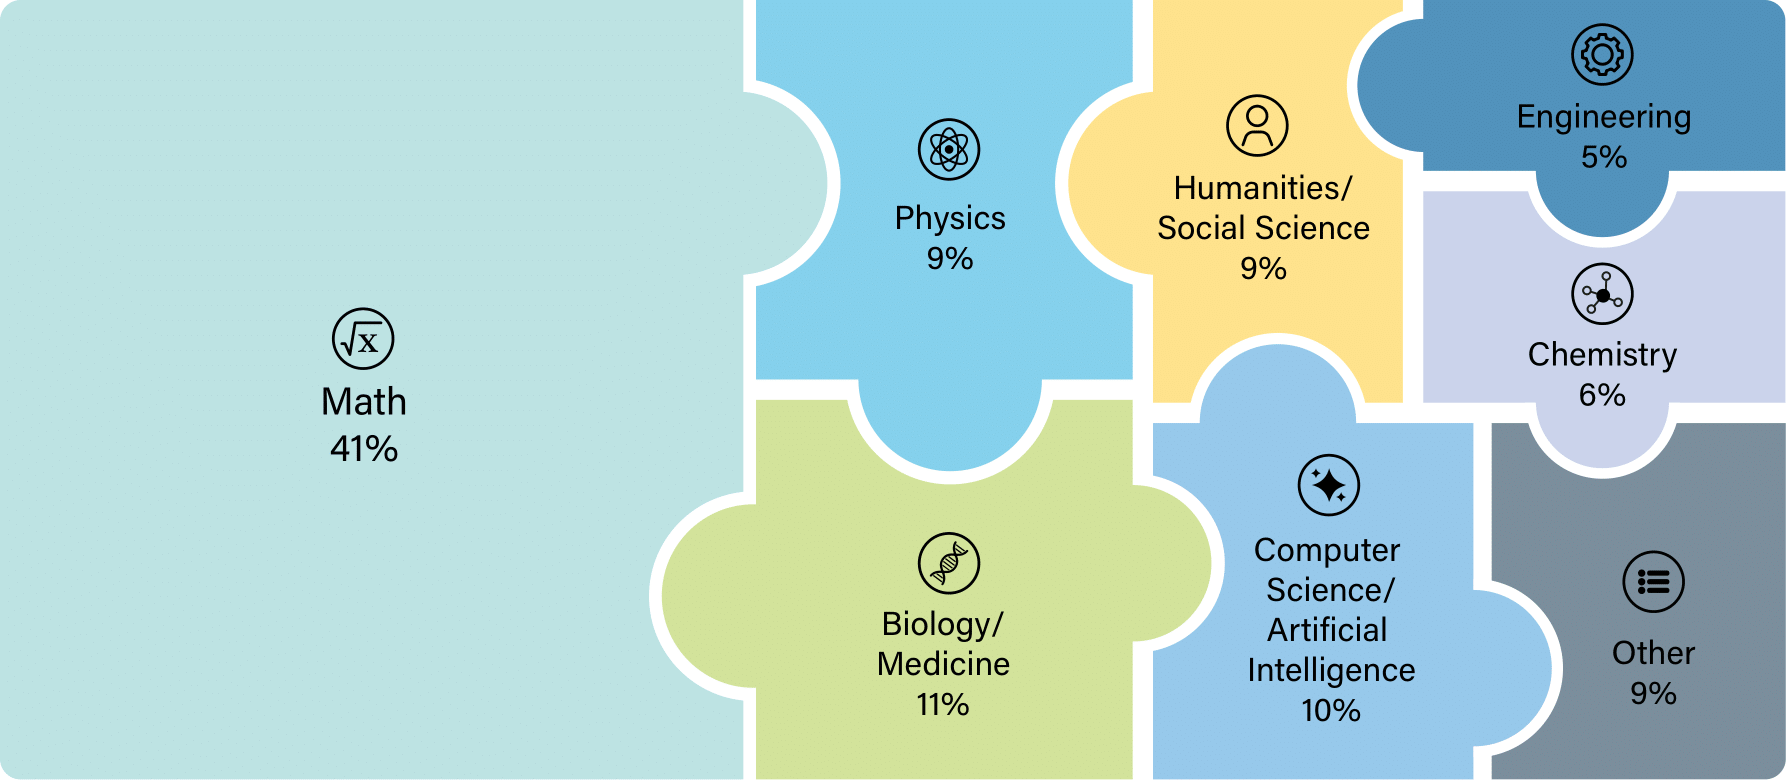
\includegraphics[width=0.8\textwidth]{.assets/dataset.png}
  \caption{Distribution of Questions in the Humanity's Last Exam Dataset \cite{phan2025humanitysexam}}
  \label{fig:dataset}
\end{figure}

\subsection{Fine-Tuning}

We selected the LLaMA Vision model for its ability to process both text and images, critical for the 4.13\% of mathematics questions with visual elements. With 11 billion parameters, it balances computational feasibility and performance, offering an open-source, resource-efficient solution for single graphics processing unit fine-tuning, unlike text-only models. Its vision-language integration aligns with trends in multimodal artificial intelligence.



Fine-tuning employs quantized low-rank adaptation, using 4-bit quantization with a normal float type and brain float 16 compute precision to reduce memory usage while preserving performance akin to full-precision models. Low-rank adapters, configured with a rank of 4, alpha of 32, and 5\% dropout, target query and value projection modules. Inputs are tokenized to a maximum length of 32 tokens, padded, and truncated as needed. To enhance mathematical reasoning, we integrate Group-Relative Policy Optimization, which eliminates the critic model and estimates baselines from group scores of multiple outputs (two completions per prompt). Rewards are computed via cosine similarity between generated completions and ground-truth answers, normalized to [0, 1], with a Kullback-Leibler penalty (beta = 0.1) ensuring alignment with the reference model.

Quantization of the 11-billion-parameter model to 4 bits with rank-4 low-rank adaptation reduces its memory footprint \( M_{\text{total}} \) as:

\begin{equation}
  M_{\text{total}} = (P \times B / 8) + A + T + D,
\end{equation}

\noindent
where \( P = 11 \times 10^9 \) parameters, \( B = 4 \) bits (0.5 bytes), \( A = 0.008 \) gigabytes (low-rank adapters), \( T = 1.5 \) gigabytes (training overhead), and \( D = 0.16 \) gigabytes (dataset). This yields \( M_{\text{total}} = (11 \times 0.5) + 0.008 + 1.5 + 0.16 = 7.168 \) gigabytes \cite{dettmers2023qloraefficientfinetuningquantized}.

Training occurs over 2 epochs with a batch size of 2 and a learning rate of \(1 \times 10^{-4}\), generating two completions per prompt (temperature 0.7, 32-token limit) using online sampling from the real-time policy model. Validated on the test set, this combined approach enhances reasoning and problem-solving efficiently, drawing on prior work demonstrating parameter-efficient gains and reward-based optimization improvements \cite{shao2024deepseekmathpushinglimitsmathematical}.

%-----------------------------------------------------------------------


\section{Expected Contributions and Metrics}
This study contributes by fine-tuning the LLaMA model with Group-Relative Policy Optimization and evaluating its ability to generalize to unseen problems in the Humanity's Last Exam dataset. We adopt the same evaluation metrics and methodology as the original Humanity's Last Exam study to ensure consistency and comparability \cite{phan2025humanitysexam}. Specifically, we focus on model accuracy, which measures the percentage of correct answers to test questions, and calibration error, which assesses the alignment between the model's predicted confidence and actual performance. These metrics are sound for evaluating reasoning and reliability, maintaining continuity with prior work while addressing our hypothesis. As this is a research proposal, we do not present results but aim to establish a framework for quantifying improvements in predictive accuracy and confidence calibration, critical for assessing adaptation to novel academic challenges.



%-----------------------------------------------------------------------


\section{Results}

Table~\ref{tab:results} presents the comparative evaluation of our approach (LLaMA + GRPO) alongside models from the Humanity's Last Exam study. The table includes two key metrics: model accuracy, which measures the ability to correctly solve unseen problems, and calibration error, which assesses the reliability of the model’s confidence estimates. Our evaluation follows a split train-evaluation framework, focusing on the model’s capacity to generalize to new and challenging problem domains.

\begin{table}[H]
\centering
\begin{tabular}{lccc}
Model                   & Accuracy (\%) ↑ & Calibration Error (\%) ↓ & Source \\
GPT-4o                  & 3.1             & 92.3                      & \cite{phan2025humanitysexam} \\
Grok-2                  & 3.9             & 90.8                      & \cite{phan2025humanitysexam} \\
Sonnet 3.5              & 4.8             & 88.5                      & \cite{phan2025humanitysexam} \\
Gemini Flash Thinking   & 7.2             & 90.6                      & \cite{phan2025humanitysexam} \\
o1                      & 8.8             & 92.8                      & \cite{phan2025humanitysexam} \\
DeepSeek-R1*            & 8.6             & 81.4                      & \cite{phan2025humanitysexam} \\
o3-mini (medium)*       & 11.1            & 91.5                      & \cite{phan2025humanitysexam} \\
o3-mini (high)*         & 14.0            & 92.8                      & \cite{phan2025humanitysexam} \\
LLaMA                   & -               & -                         &  \\
LLaMA + GRPO (ours)     & -               & -                         &  \\
\\
\end{tabular}
\caption{
  Comparative Evaluation of Models on the Humanity's Last Exam Benchmark.
  *Model is not multi-modal, evaluated on text-only subset.
  }
  \label{tab:results}
\end{table}


%-----------------------------------------------------------------------

\section{Discussion}
TBD

% Multiple frameworks exist for fine-tuning large language models, offering diverse quantization and optimization strategies. However, our exploration of popular solutions revealed significant limitations stemming from restricted hardware support and compatibility issues. Notably, many libraries lack support for central processing unit training, a constraint compounded by the limited graphics processing unit memory available to us (operating with CUDA 12.6). Alternative solutions often required stacking disparate frameworks to achieve the desired quantization and fine-tuning outcomes, yet cross-compatibility with our graphics processing unit’s CUDA version proved elusive for several libraries, rendering straightforward implementations unfeasible.

% Our choice of quantized low-rank adaptation was further informed by challenges in available implementations. Despite claims from LLaMA documentation that multiple PyTorch and Hugging Face methods support quantized low-rank adaptation and quantization-aware training, only one configuration proved viable for training our model \cite{llama_quantization_2025}. Other options, such as those provided by TorchAO and Hugging Face Transformers, were primarily suited for inference rather than fine-tuning. 




% Pytorch quantization with TorchAO
% The TorchAO library offers several methods for quantization, each with different schemes for how the activations and weights are quantized. We distinguish between two main types of quantization: weight only quantization and dynamic quantization.
% For weight only quantization, we support 8-bit and 4-bit quantization. The 4-bit quantization also has GPTQ support for improved accuracy, which requires calibration but has the same final performance.
% For dynamic quantization, we support 8-bit activation quantization and 8-bit weight quantization. We also support this type of quantization with smoothquant for improved accuracy, which requires calibration and has slightly worse performance.
% Additionally, the library offers a simple API to test different methods and automatic detection of the best quantization for a given model, known as autoquantization. This API chooses the fastest form of quantization out of the 8-bit dynamic and 8-bit weight only quantization. It first identifies the shapes of the activations that the different linear layers see, then benchmarks these shapes across different types of quantized and non-quantized layers in order to pick the fastest one. Also, it composes with torch.compile() to generate the fast kernels. For additional information on torch.compile, please see this general tutorial.
% Note: This library is in beta phase and in active development; API changes are expected.
% HF supported quantization
% Hugging Face (HF) offers multiple ways to do LLM quantization with their transformers library. For additional guidance and examples on how to use each of these beyond the brief summary presented here, please refer to their quantization guide and the transformers quantization configuration documentation. The LLaMA-cookbook code uses bitsandbytes 8-bit quantization to load the models, both for inference and fine-tuning. (See below for more information about using the bitsandbytes library with LLaMA. )
% TorchAO
% The Hugging Face Transformers library supports TorchAO (PyTorch Architecture Optimization). As described above, TorchAO enables you to quantize and sparsify: weights, gradients, optimizers, and activations. TorchAO supports custom data types and optimizations. You can use TorchAO for both training and inference.
% from transformers import TorchAoConfig, AutoModelForCausalLM, AutoTokenizer
% See the Hugging Face page for more information and examples that describe their support for TorchAO.
% Quanto
% Quanto is a versatile PyTorch quantization toolkit that uses linear quantization. It provides features such as weights quantization, activation quantization, and compatibility with various devices and modalities. It supports quantization-aware training and is easy to integrate with custom kernels for specific devices. More details can be found in the announcement blog, GitHub repository, and HF guide.
% AQLM
% Additive Quantization of Language Models (AQLM) is a compression method for LLM. It quantizes multiple weights together, taking advantage of interdependencies between them. AQLM represents groups comprising 8 to16 weights each as a sum of multiple vector codes. This library supports fine-tuning its quantized models with Parameter-Efficient Fine-Tuning and LoRA by integrating into HF's PEFT library as well. More details can be found in the GitHub repository.
% AWQ
% Activation-aware Weight Quantization (AWQ) preserves a small percentage of weights that are important for LLM performance, reducing quantization loss. This allows models to run in 4-bit precision without experiencing performance degradation. Transformers support loading models quantized with the llm-awq and autoawq libraries. More details on how to load them with the Transformers library can be found in the HF guide.
% AutoGPTQ
% The AutoGPTQ library implements the GPTQ algorithm, a post-training quantization technique where each row of the weight matrix is quantized independently. These weights are quantized to int4, but they’re restored to fp16 on the fly during inference, saving memory usage by 4x. More details can be found in the GitHub repository.
% BitsAndBytes
% BitsAndBytes is an easy option for quantizing a model to 8-bit and 4-bit. The library supports any model in any modality, as long as it supports loading with Hugging Face Accelerate and contains torch.nn.Linear layers. It also provides features for offloading weights between the CPU and GPU to support fitting very large models into memory, adjusting the outlier threshold for 8-bit quantization, skipping module conversion for certain models, and fine-tuning with 8-bit and 4-bit weights. For 4-bit models, it allows changing the compute data type, using the Normal Float 4 (NF4) data type for weights initialized from a normal distribution, and using nested quantization to save additional memory at no additional performance cost. More details can be found in the HF guide.



%-----------------------------------------------------------------------


\section{Conclusion and Future Work}
TBD
% - Grow the dataset with new unique problems
% - Explore ways to generate new problems with the dataset and generative models
% - Potentially fine-tune on MATH dataset
% - Could GRPO with classic math datasets improve the model's performance against its baseline?
% - Better support for QLoRA with new, more complete frameworks

%-----------------------------------------------------------------------


\section{Acknowledgements}
The author acknowledges the support of the School of Computing at the University of Leeds and extends gratitude to the developers of QLoRA, GRPO, and the HLE dataset for making their resources publicly available.


%-----------------------------------------------------------------------


\section{Data Access Statement}
The code and results used in this study are openly accessible at {\it \href{https://github.com/pre63/grpo-fine-tuning-LLaMA-study}{this repository}}. It contains all the scripts, configurations, and datasets analysis necessary to reproduce the experiments and validate the findings presented in this work.


%-----------------------------------------------------------------------


\printbibliography


%-----------------------------------------------------------------------

\section{Appendix}

\subsection{Appendix A: Dataset Description}

\begin{center}
  \begin{table}[H]
\centering
\begin{tabular}{lrrrr}
\toprule
Category & Questions & Min Test Size & Min Test \% & Train \% \\
\midrule
Biology/Medicine & 303 & 143 & 47.260000 & 52.740000 \\
Chemistry & 170 & 105 & 61.560000 & 38.440000 \\
Computer Science/AI & 258 & 132 & 51.290000 & 48.710000 \\
Engineering & 130 & 88 & 67.720000 & 32.280000 \\
Humanities/Social Science & 235 & 126 & 53.630000 & 46.370000 \\
Math & 1106 & 218 & 19.670000 & 80.330000 \\
Other & 258 & 132 & 51.290000 & 48.710000 \\
Physics & 240 & 127 & 53.100000 & 46.900000 \\
\bottomrule
\end{tabular}
\vspace{0.2cm}
\caption{Statistics by Category for cais/hle Test Split (90\% CI, 5\% Error)}
\label{tab:split_analysis}
\end{table}
 
\end{center}

\begin{center}
  \begin{table}[H]
\centering
\begin{tabular}{lrrrrr}
\toprule
Category & Questions & Train \% & Test \% & \% Image & \% Exact Match \\
\midrule
Biology/Medicine & 303 & 52.81 & 47.19 & 19.58 & 48.25 \\
Chemistry & 170 & 38.24 & 61.76 & 38.10 & 75.24 \\
Computer Science/AI & 258 & 48.84 & 51.16 & 6.82 & 69.70 \\
Engineering & 130 & 32.31 & 67.69 & 46.59 & 72.73 \\
Humanities/Social Science & 235 & 46.38 & 53.62 & 11.11 & 59.52 \\
Math & 1106 & 80.29 & 19.71 & 4.13 & 91.28 \\
Other & 258 & 48.84 & 51.16 & 22.73 & 75.00 \\
Physics & 240 & 47.08 & 52.92 & 6.30 & 84.25 \\
\bottomrule
\end{tabular}
\vspace{0.2cm}
\caption{Dataset Train/Test Split by Category}
\label{tab:split_statistics}
\end{table}
 
\end{center}

\begin{center}
  \begin{table}[H]
\centering
\begin{tabular}{llll}
\toprule
Category & Text Tokens  & Image Size (MB) & Images \\
\midrule
Biology/Medicine & $\downarrow$11 - $\uparrow$3008 257.13$\mu$ $\pm$344.08$\sigma$ & 0.3582$\mu$ $\pm$0.3318$\sigma$ & 19.47\% \\
Chemistry & $\downarrow$16 - $\uparrow$1699 186.07$\mu$ $\pm$259.06$\sigma$ & 0.0655$\mu$ $\pm$0.0967$\sigma$ & 36.47\% \\
Computer Science/AI & $\downarrow$15 - $\uparrow$5052 420.34$\mu$ $\pm$648.82$\sigma$ & 0.2335$\mu$ $\pm$0.3776$\sigma$ & 5.81\% \\
Engineering & $\downarrow$14 - $\uparrow$8972 396.45$\mu$ $\pm$919.56$\sigma$ & 0.1733$\mu$ $\pm$0.2037$\sigma$ & 40.0\% \\
Humanities/Social Science & $\downarrow$15 - $\uparrow$1294 201.03$\mu$ $\pm$227.64$\sigma$ & 0.3205$\mu$ $\pm$0.3624$\sigma$ & 10.64\% \\
Math & $\downarrow$15 - $\uparrow$13518 216.81$\mu$ $\pm$483.85$\sigma$ & 0.145$\mu$ $\pm$0.211$\sigma$ & 4.07\% \\
Other & $\downarrow$11 - $\uparrow$7156 174.16$\mu$ $\pm$478.07$\sigma$ & 0.3883$\mu$ $\pm$0.4474$\sigma$ & 22.48\% \\
Physics & $\downarrow$11 - $\uparrow$7313 248.2$\mu$ $\pm$520.54$\sigma$ & 0.1423$\mu$ $\pm$0.253$\sigma$ & 5.83\% \\
\bottomrule
\end{tabular}
\vspace{0.2cm}
\caption{Dataset Description by Category for cais/hle Test Split}
\label{tab:dataset_description}
\end{table}
 
\end{center}

\end{document}
